\documentclass{beamer}
\usetheme{Singapore}
\usepackage[utf8]{inputenc}
\usecolortheme{crane}
\usepackage{graphicx}
\usepackage{iwona}
\usepackage{standalone}
\usepackage{tikz}
\usetikzlibrary{arrows}
\usetikzlibrary{decorations.markings}
\usetikzlibrary{calc}
\usetikzlibrary{shapes,snakes}
\usepackage{amsmath}
\usepackage{amsfonts}
\usepackage{amsthm}
\usepackage{mathtools}
\usepackage{tcolorbox}
\usepackage{float}
\usepackage{bm}
% \usepackage{minted}

\definecolor{lightblue}{RGB}{124,190,255}
\definecolor{darkgreen}{RGB}{24,145,0}
\definecolor{darkorange}{RGB}{220,110,0}



\beamertemplatenavigationsymbolsempty
\setbeamerfont{caption}{size=\tiny}


\title
{Phoenix Mathematics Summer School 2017}
\author{Geraint Ian Palmer}
\date{}
\titlegraphic{
\includegraphics[width=2.35cm]{cflogo}}



\begin{document}

\frame{\titlepage}

\begin{frame}
\begin{center}
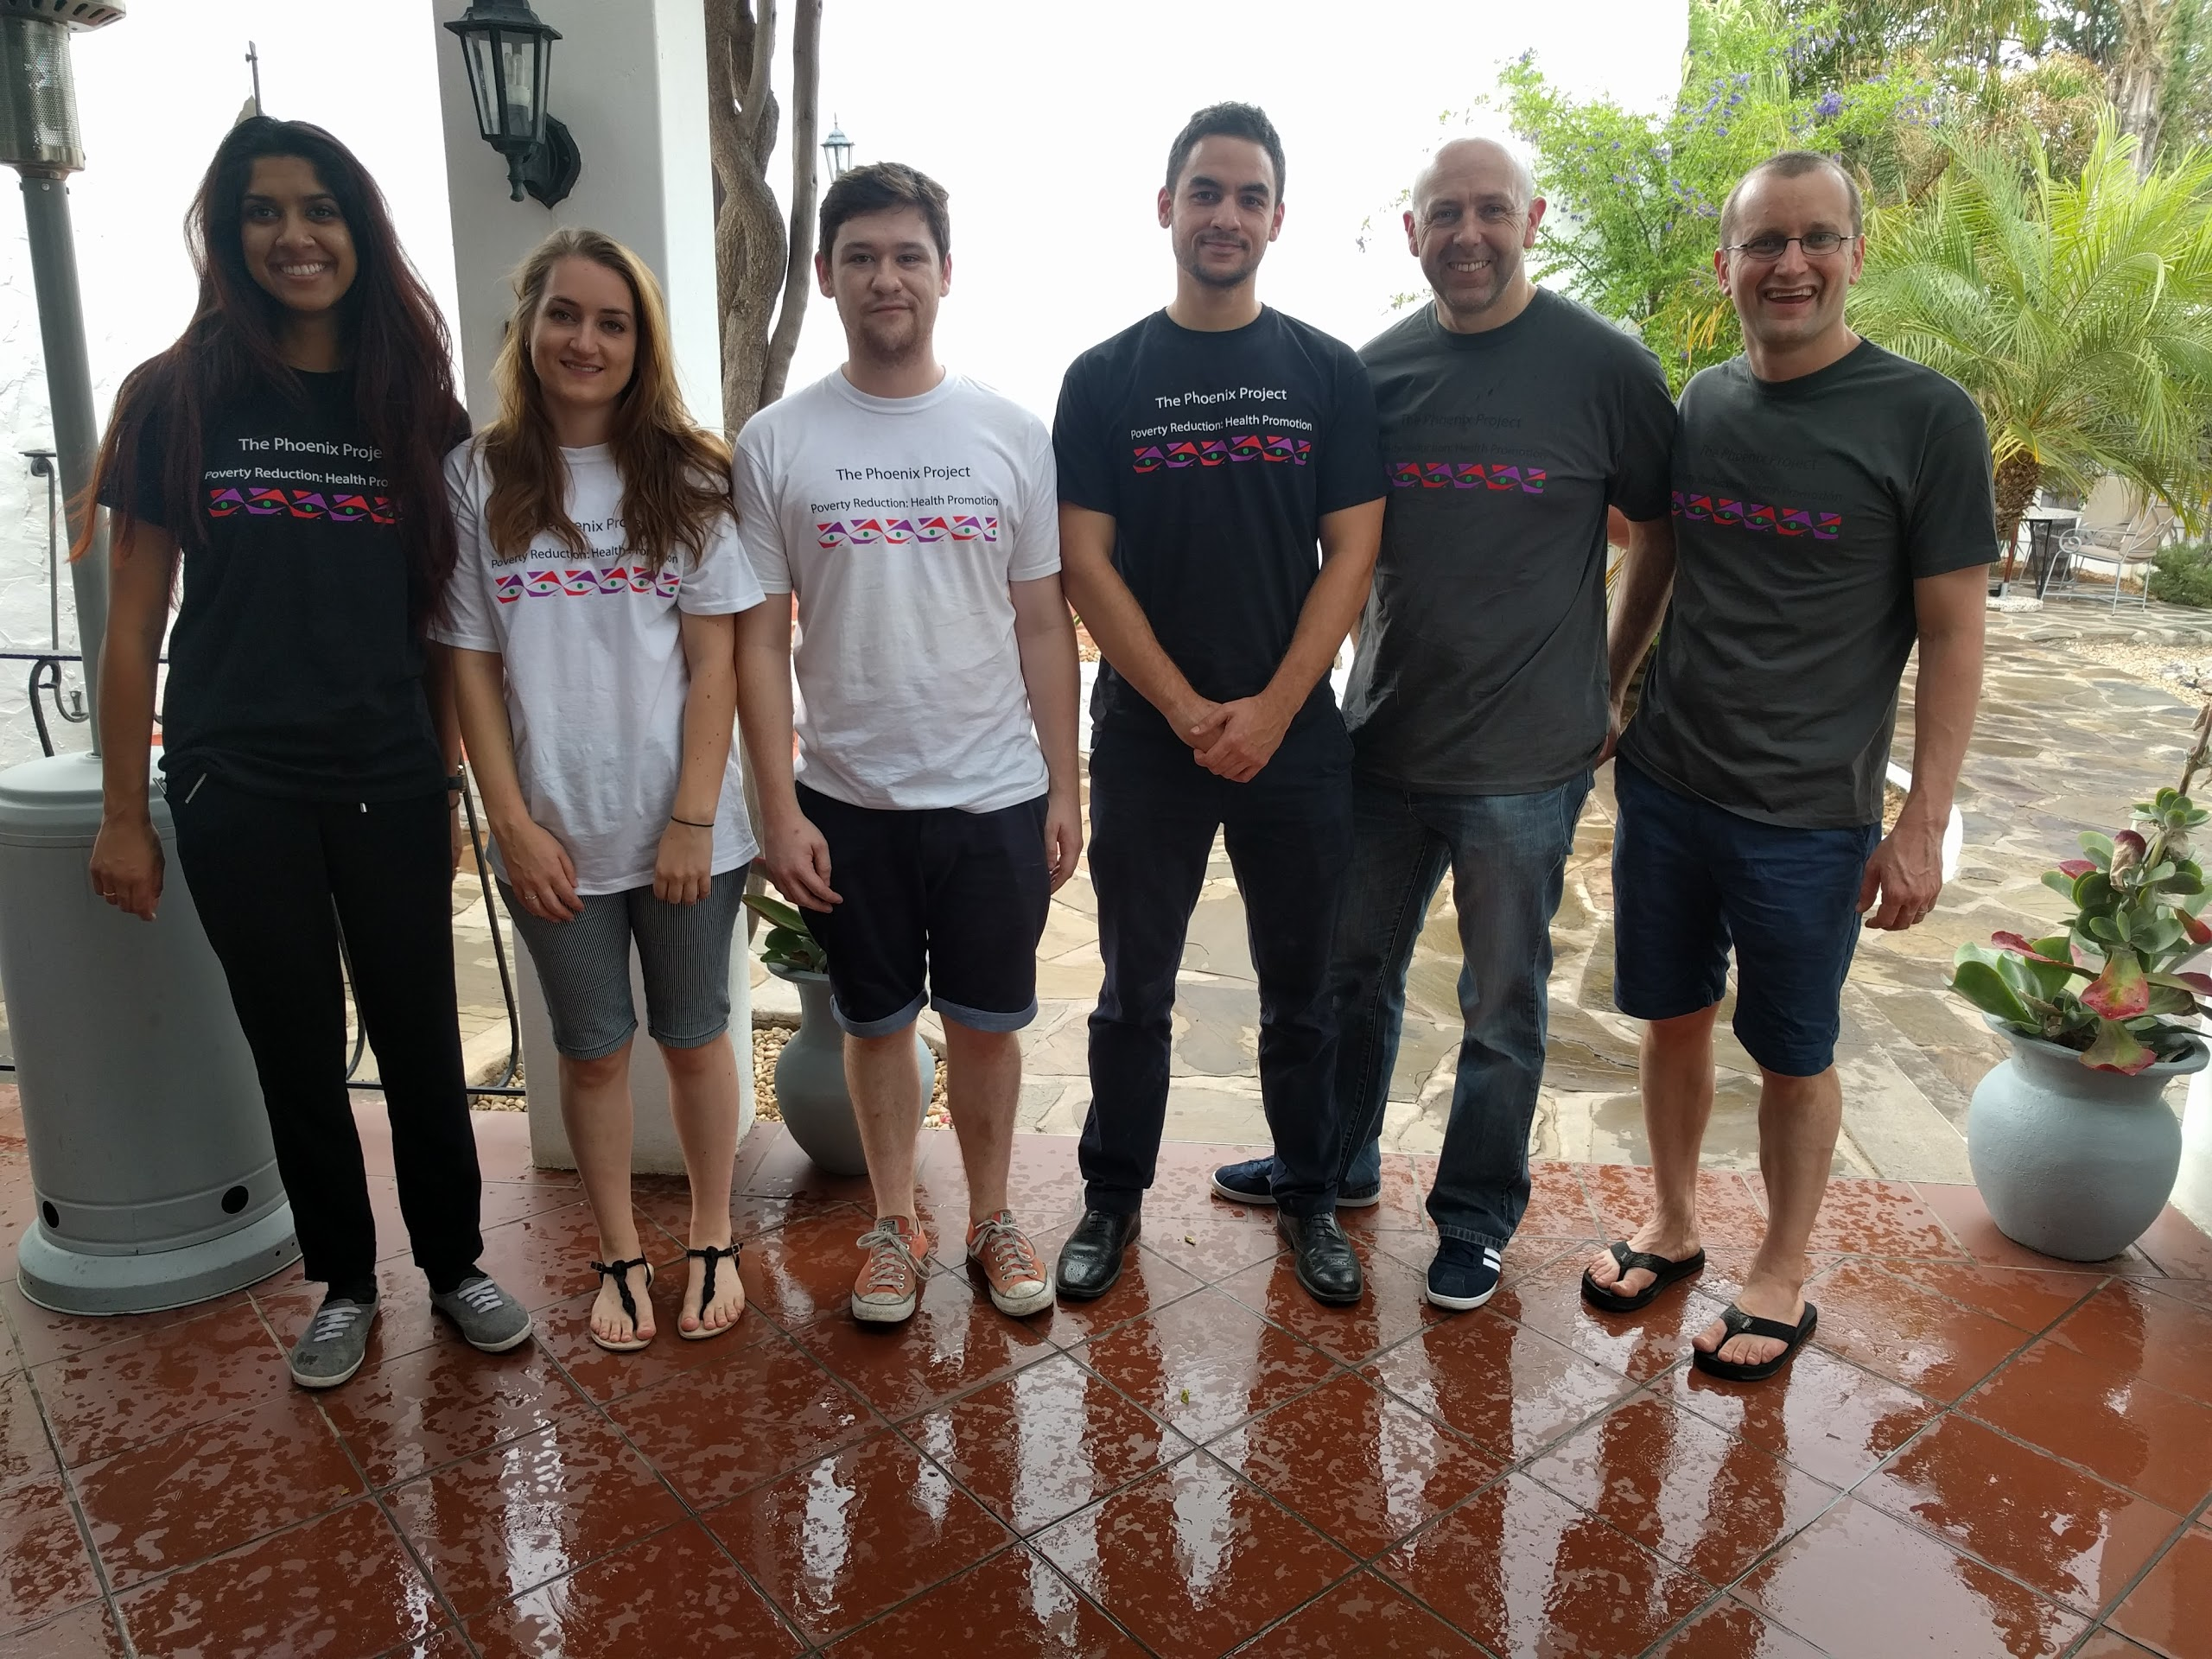
\includegraphics[width=0.85\textwidth]{all_tshirt}
\end{center}
\end{frame}

\begin{frame}
\begin{center}
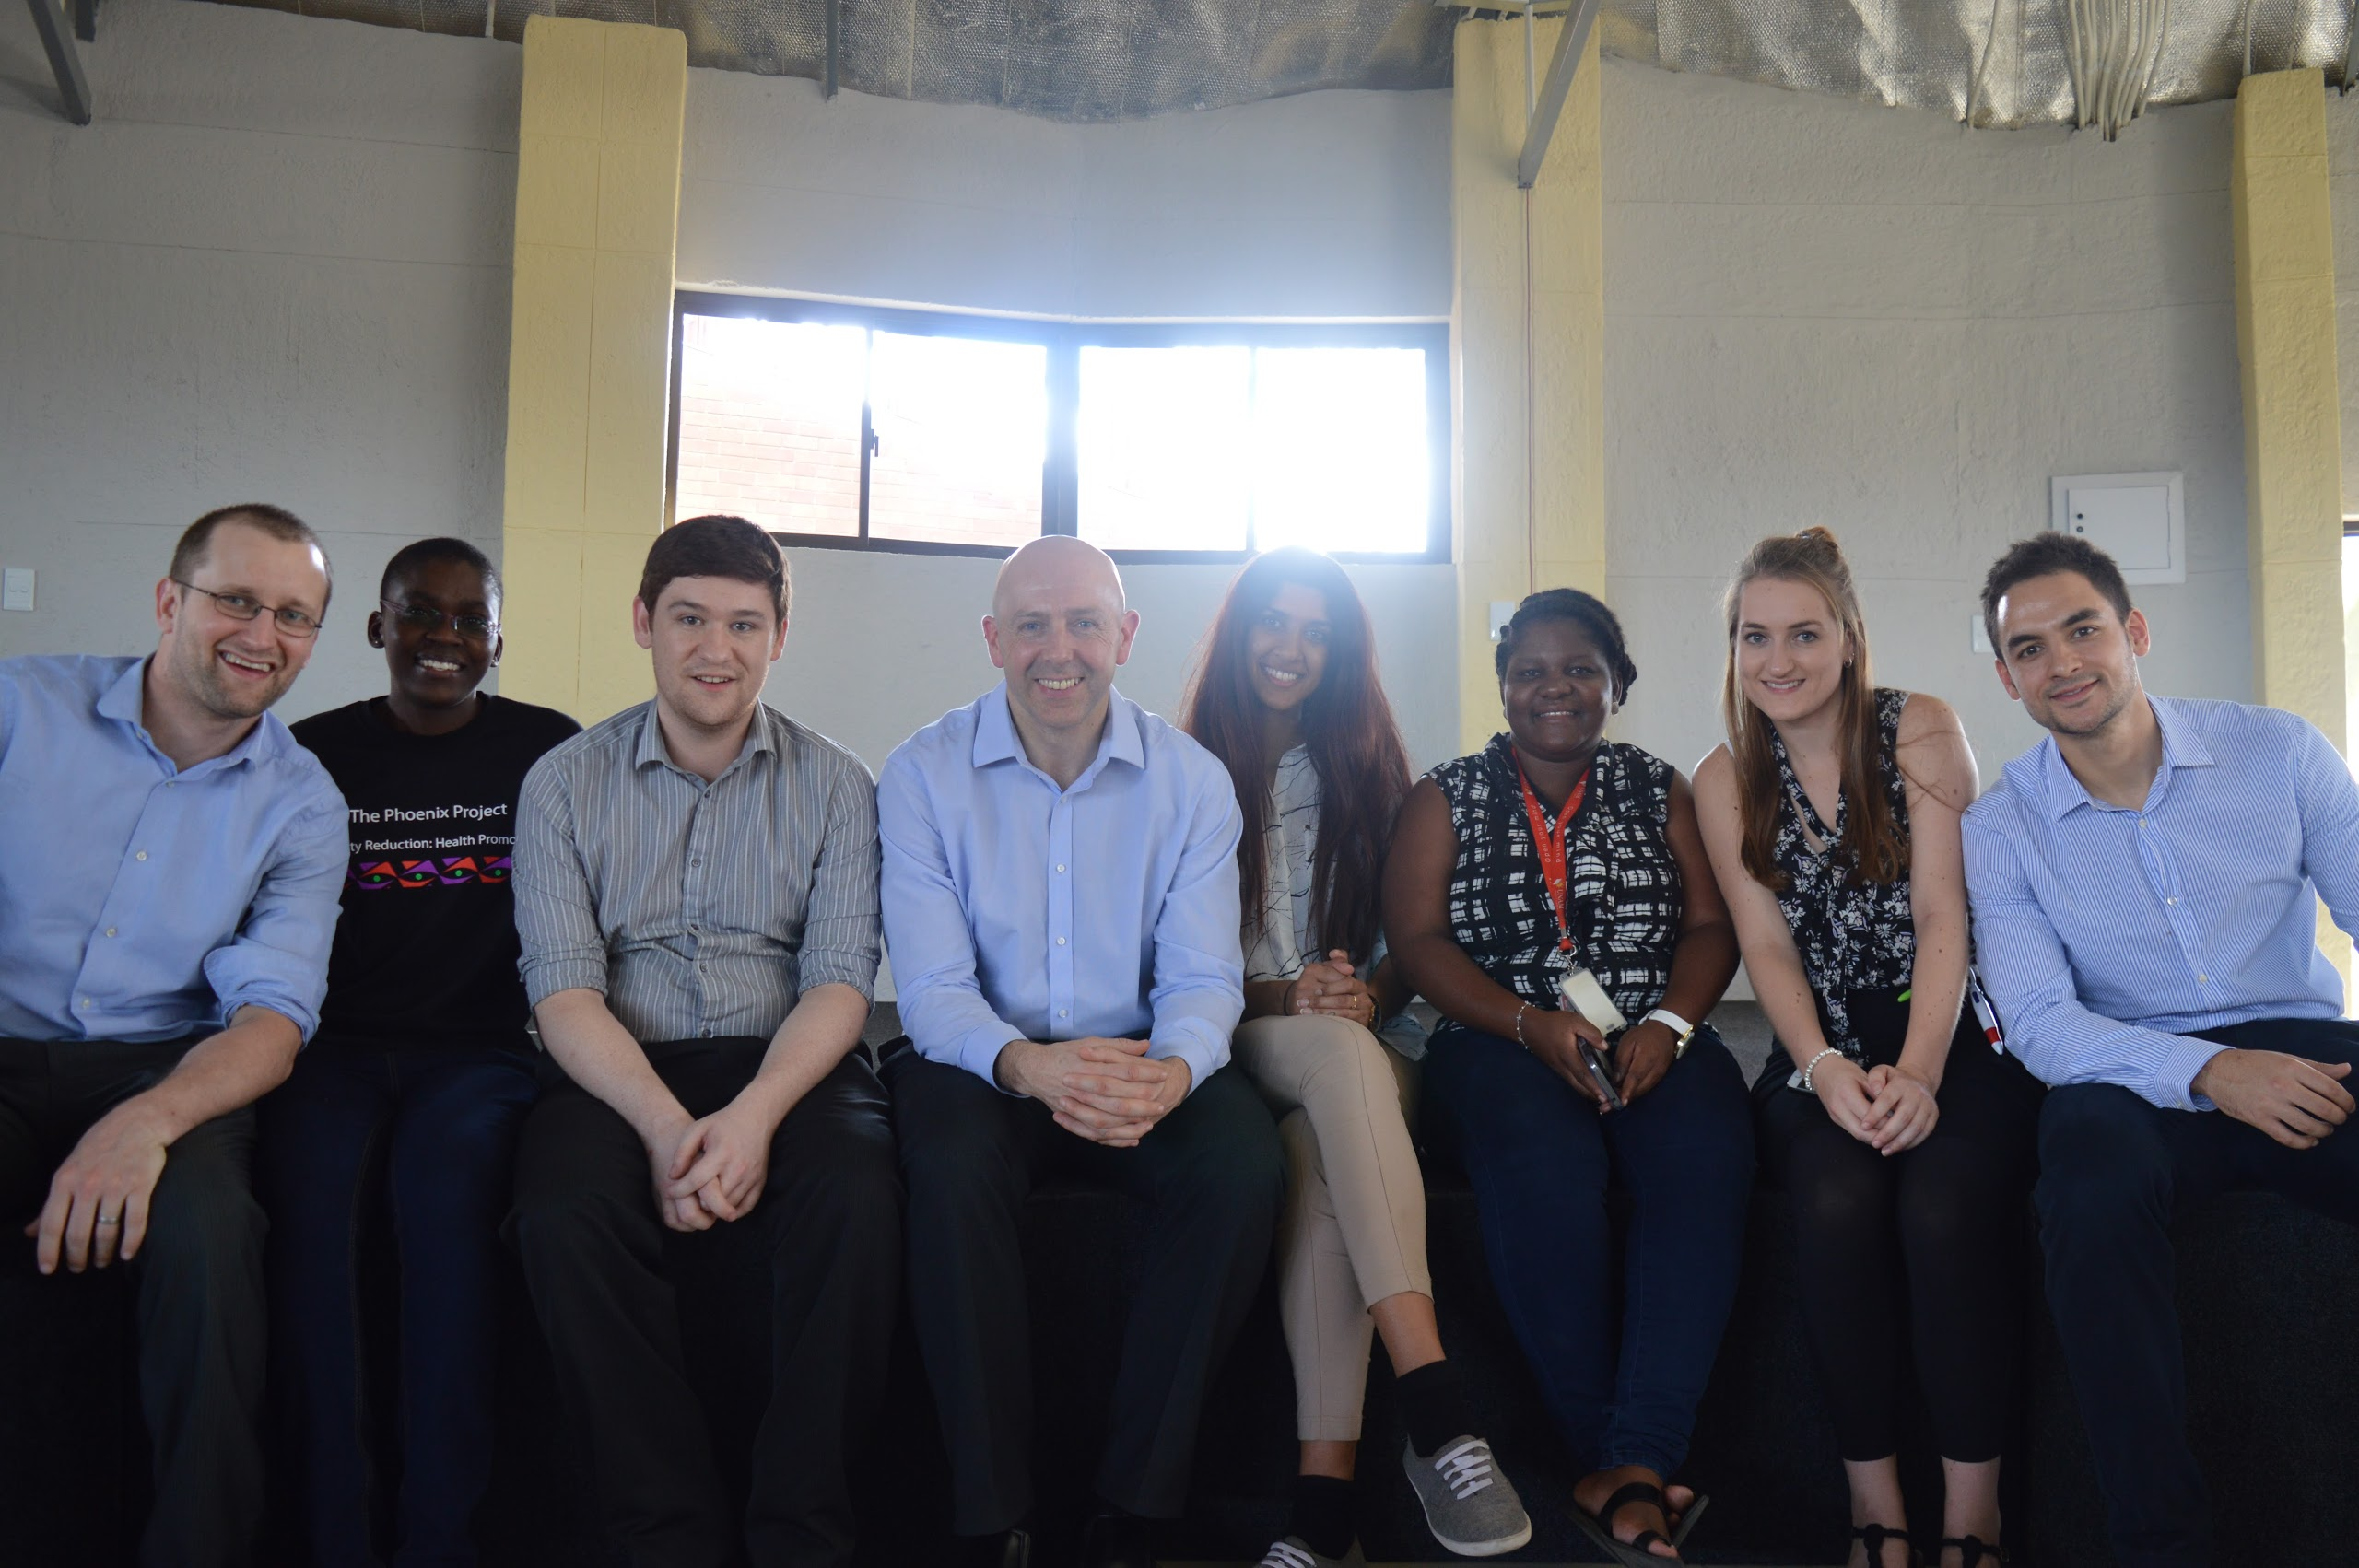
\includegraphics[width=\textwidth]{angelasaara}
\end{center}
\end{frame}

\begin{frame}
\begin{center}
\includegraphics[width=\textwidth]{teaching_collage}
\end{center}
\end{frame}

\begin{frame}
\begin{center}
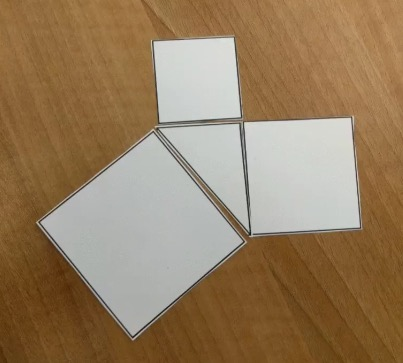
\includegraphics[width=0.31\textwidth]{pythag1}
\hspace{5mm}
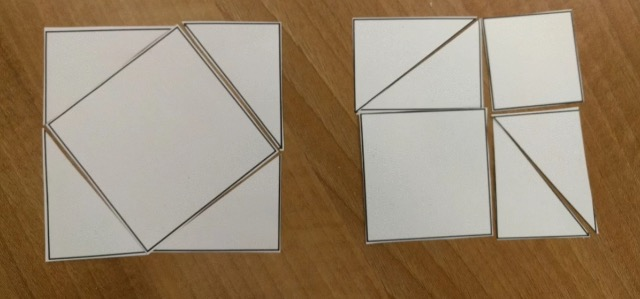
\includegraphics[width=0.6\textwidth]{pythag2}
\end{center}
\end{frame}

\begin{frame}
\begin{center}
\includegraphics[width=\textwidth]{present_collage}
\end{center}
\end{frame}

\begin{frame}
\begin{center}
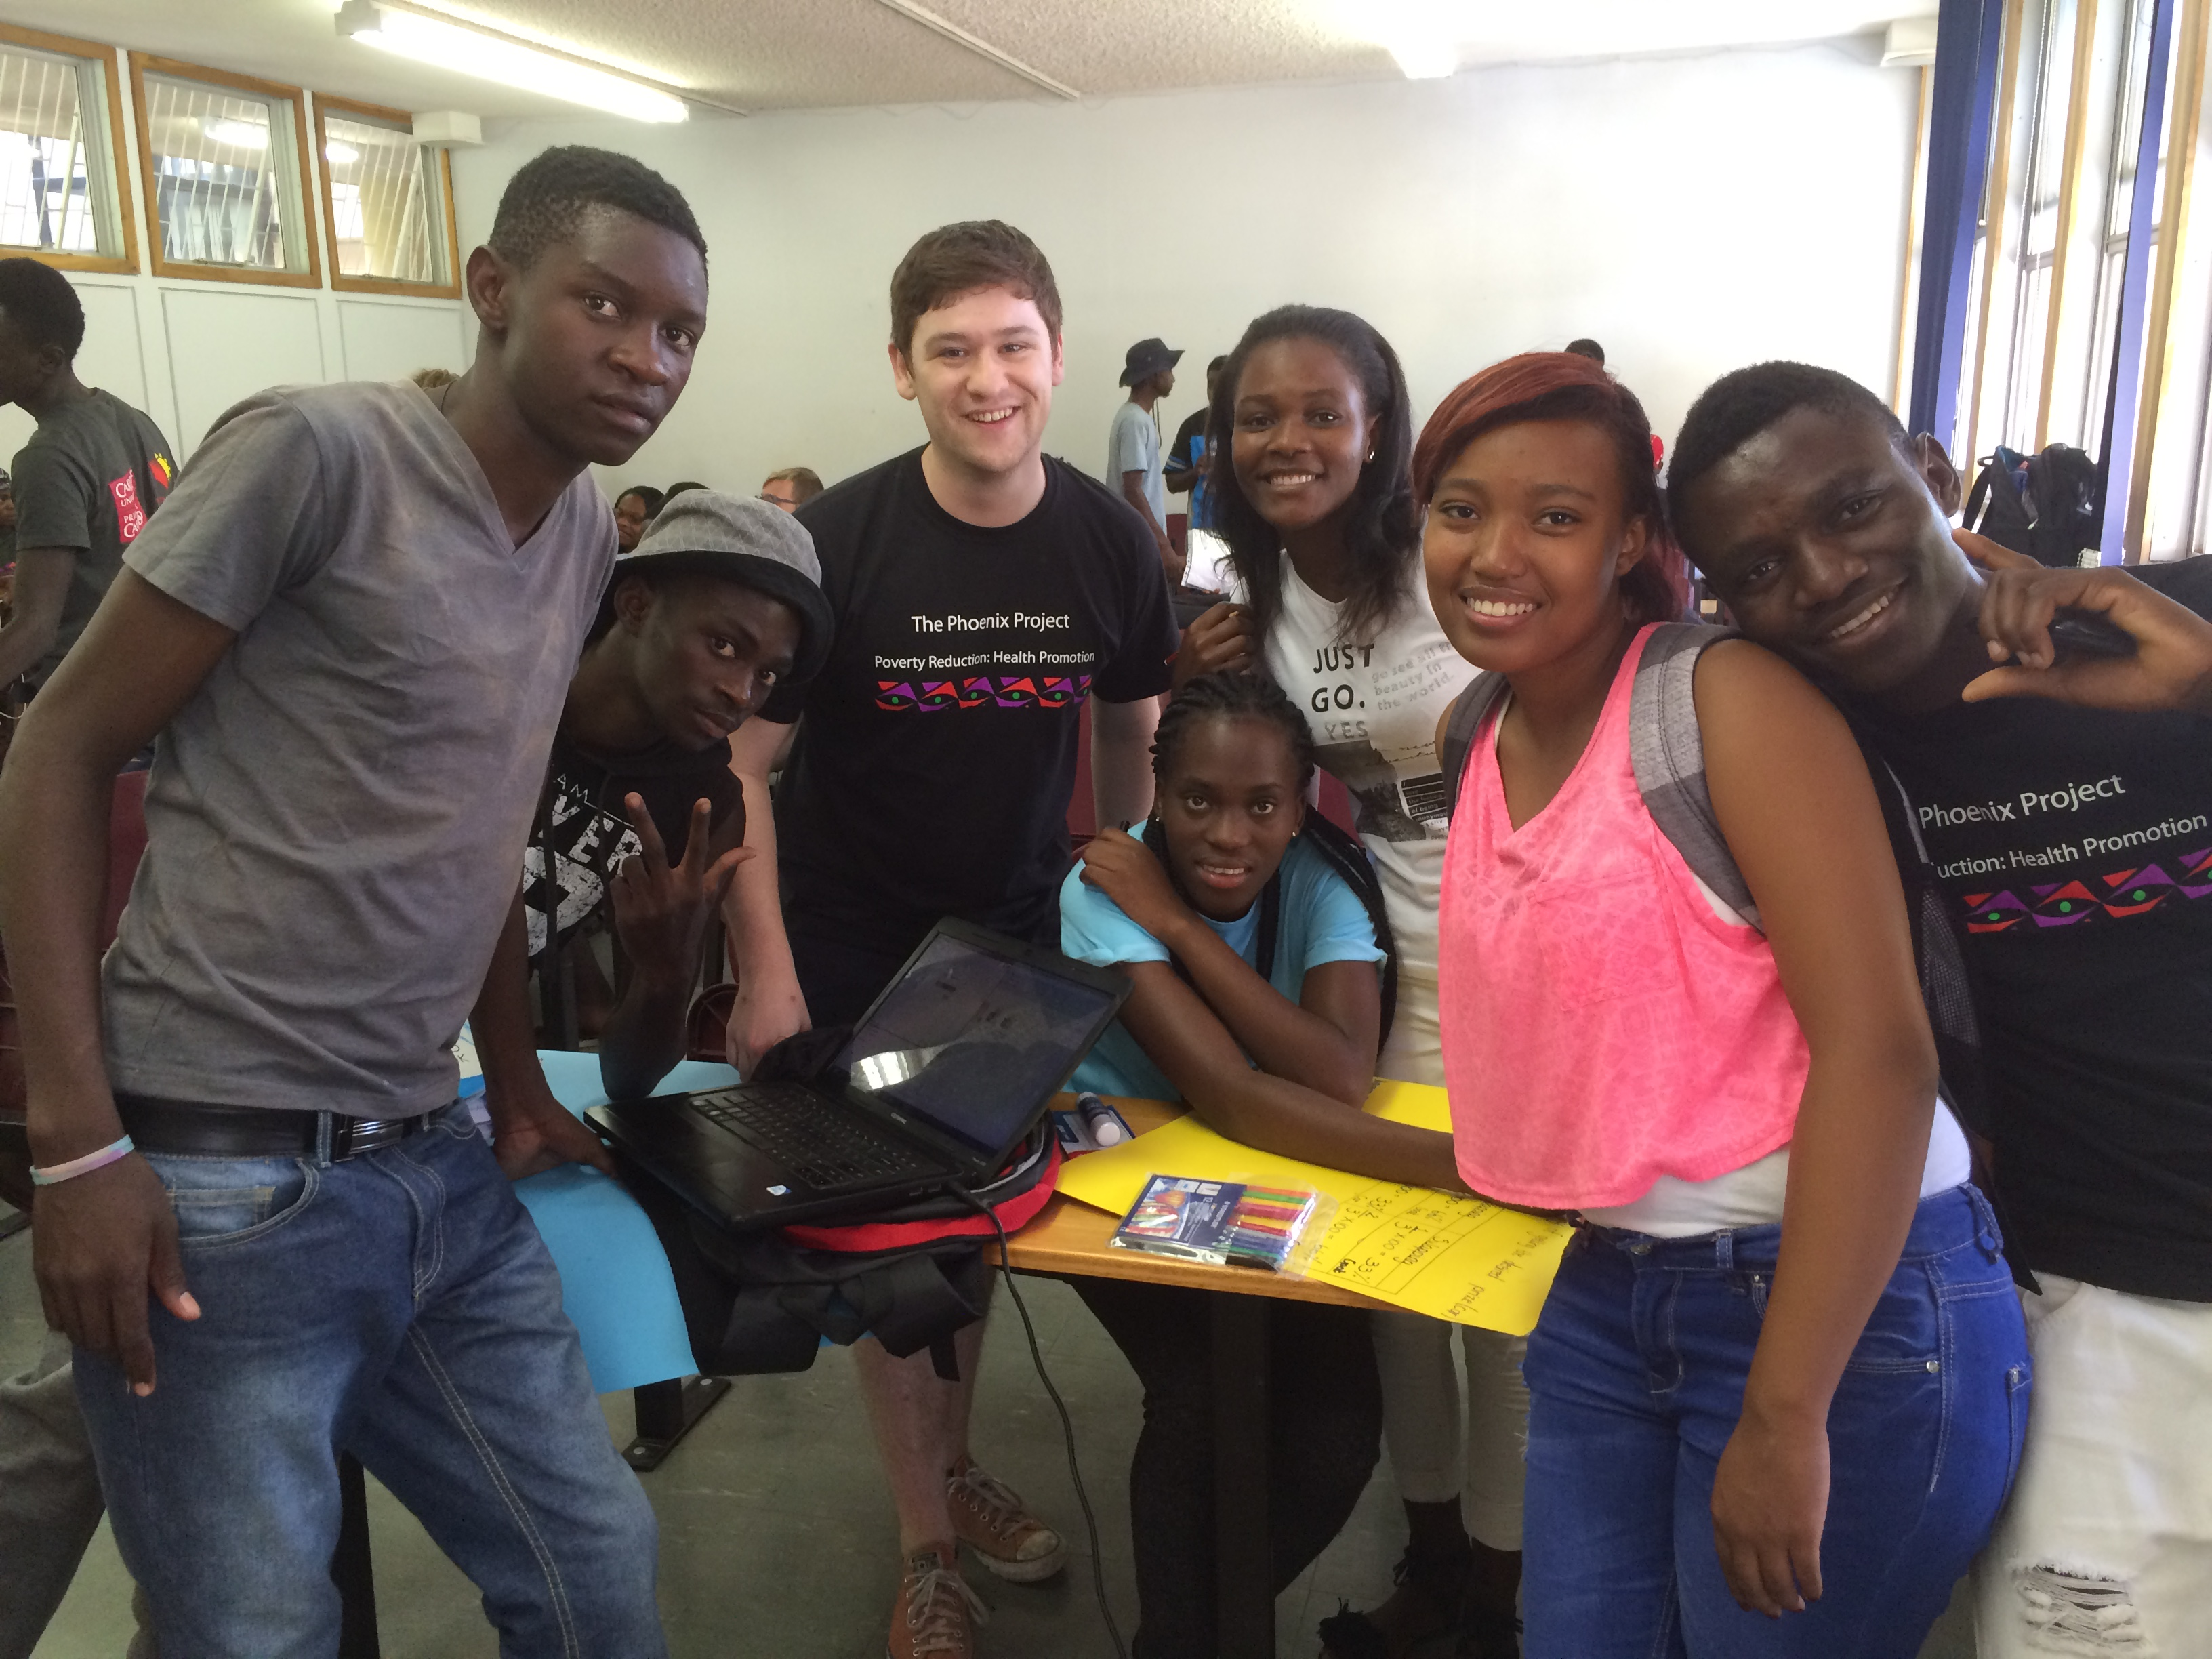
\includegraphics[width=0.48\textwidth]{proj1}
\end{center}
\begin{center}
\includegraphics[width=0.48\textwidth]{proj2}
\end{center}
\end{frame}


\begin{frame}
\begin{center}
\includegraphics[width=\textwidth]{basketball_collage}
\end{center}
\end{frame}

\begin{frame}
\begin{center}
\includegraphics[width=0.85\textwidth]{safari_collage}
\end{center}
\end{frame}


\begin{frame}
\begin{center}
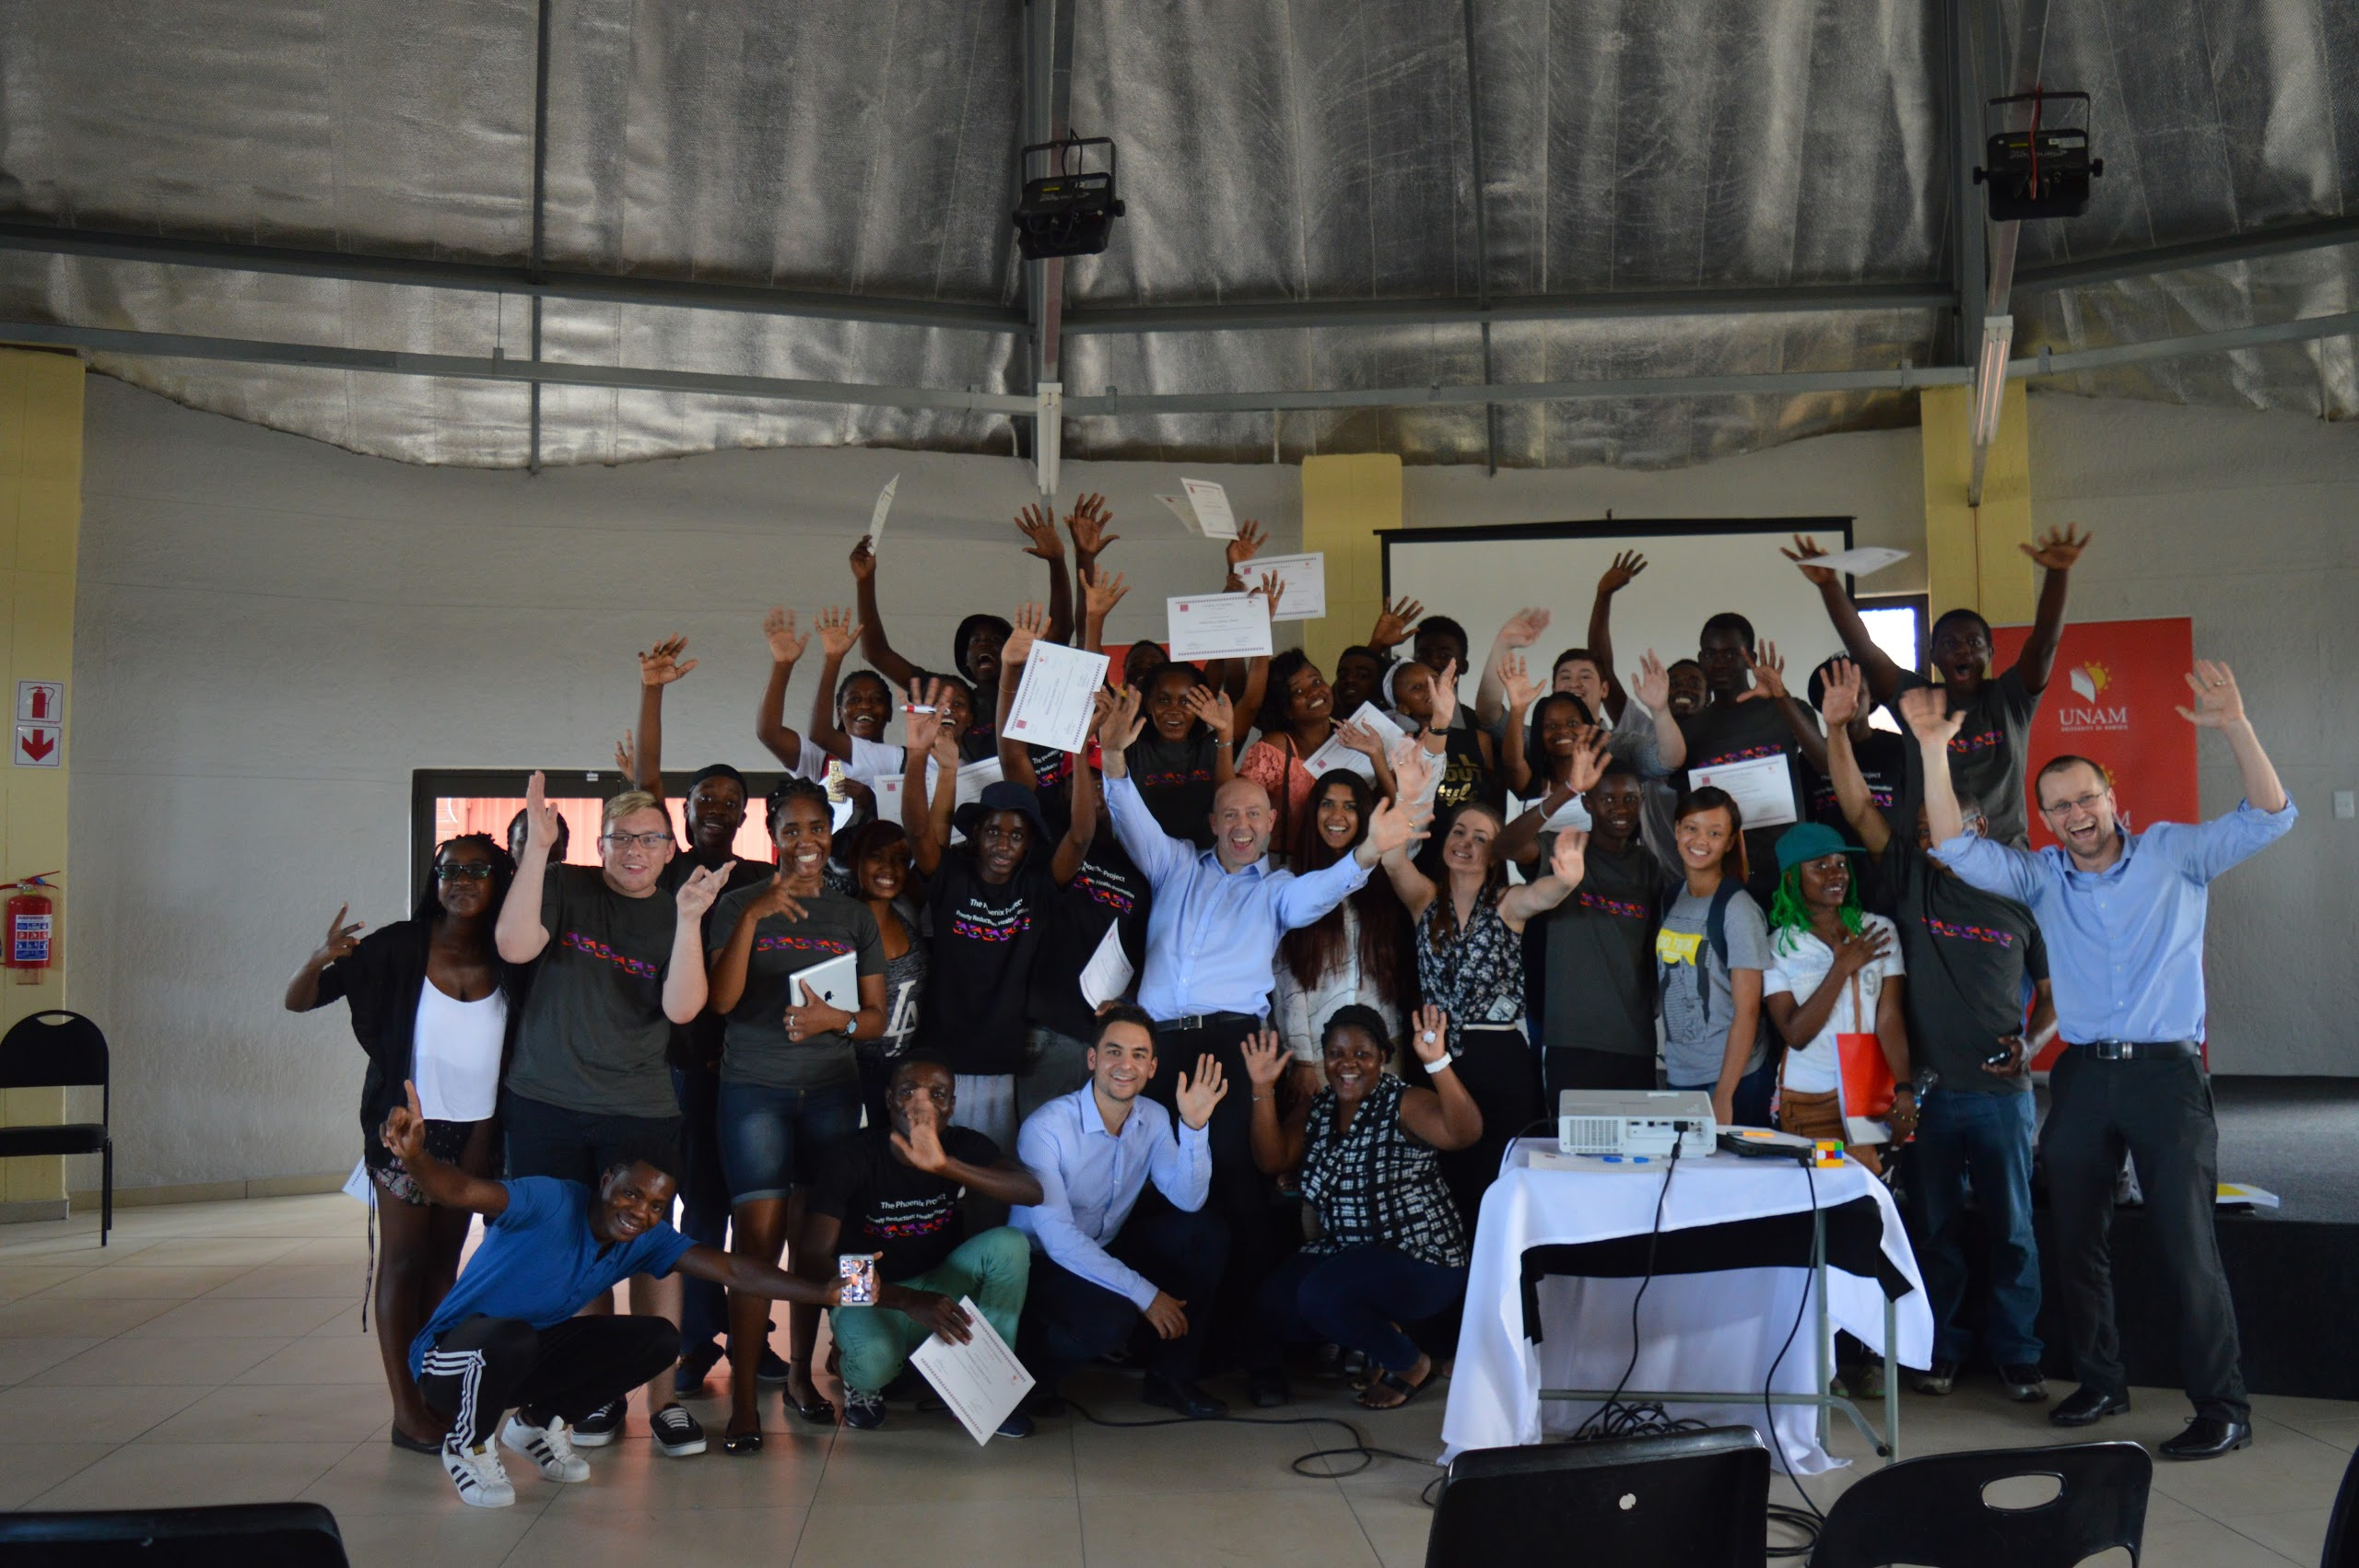
\includegraphics[width=\textwidth]{end}
\end{center}
\end{frame}


\end{document}
